
\section{Method}
\label{our_work}
In this section, we investigate the critical connection between the parameter $\beta$ and the quality of pairwise data in optimizing DPO. We present empirical evidence demonstrating the effect of $\beta$ settings on DPO performance across datasets of varying quality. Our proposed method, $\beta$-DPO, introduces dynamic calibration of $\beta$ and a data filtering mechanism tailored to improve DPO's effectiveness across diverse data conditions.
\subsection{Motivation: The Impact of Pairwise Data Quality on $\beta$ Selection}
\label{motivation_sec}
Scrutinizing Equation \eqref{eq:DPO2}, we argue that DPO's effectiveness critically hinges on two factors: the choice of $\beta$ and the quality of pairwise data. Here, we conduct experiments to demonstrate the influence of variations in $\beta$ and data quality on DPO, pivotal for its effective real-world application.

\textbf{Datasets.} 
We utilize the Anthropic HH dataset \cite{Bai2022training} for our experimental analysis, which contains approximately 170,000 dialogues between humans and an automated assistant. In this dataset, a human inquiry, denoted as $\xb$, is paired with two responses $(\yb_w, \yb_l)$, where $\yb_w$ represents the response favored by the human annotator, while $y_l$ is the alternate response. Notably, the alternate response $y_l$ retains informational value, making this dataset high-quality with minimal discrepancies between the response pairs, which we classify as a \emph{low gap} dataset.
To further explore the impact of data quality on DPO, we construct a synthetic dataset, referred to as the \emph{high gap} dataset. This dataset differs from the \emph{low gap} dataset by introducing a greater disparity between responses. Specifically, the alternative response $y_l$ is generated by a Supervised FineTuned (SFT) Pythia-2.8B model, while the preferred response $y_w$ remains consistent with the original dataset.
We also combine the two datasets in equal proportion to create a \emph{mixed gap} dataset, with each contributing 50\%, to incorporate the characteristics of both the \emph{low gap} and \emph{high gap} datasets.

 \begin{figure}[t]
    \vspace{-10pt}
    \centering
    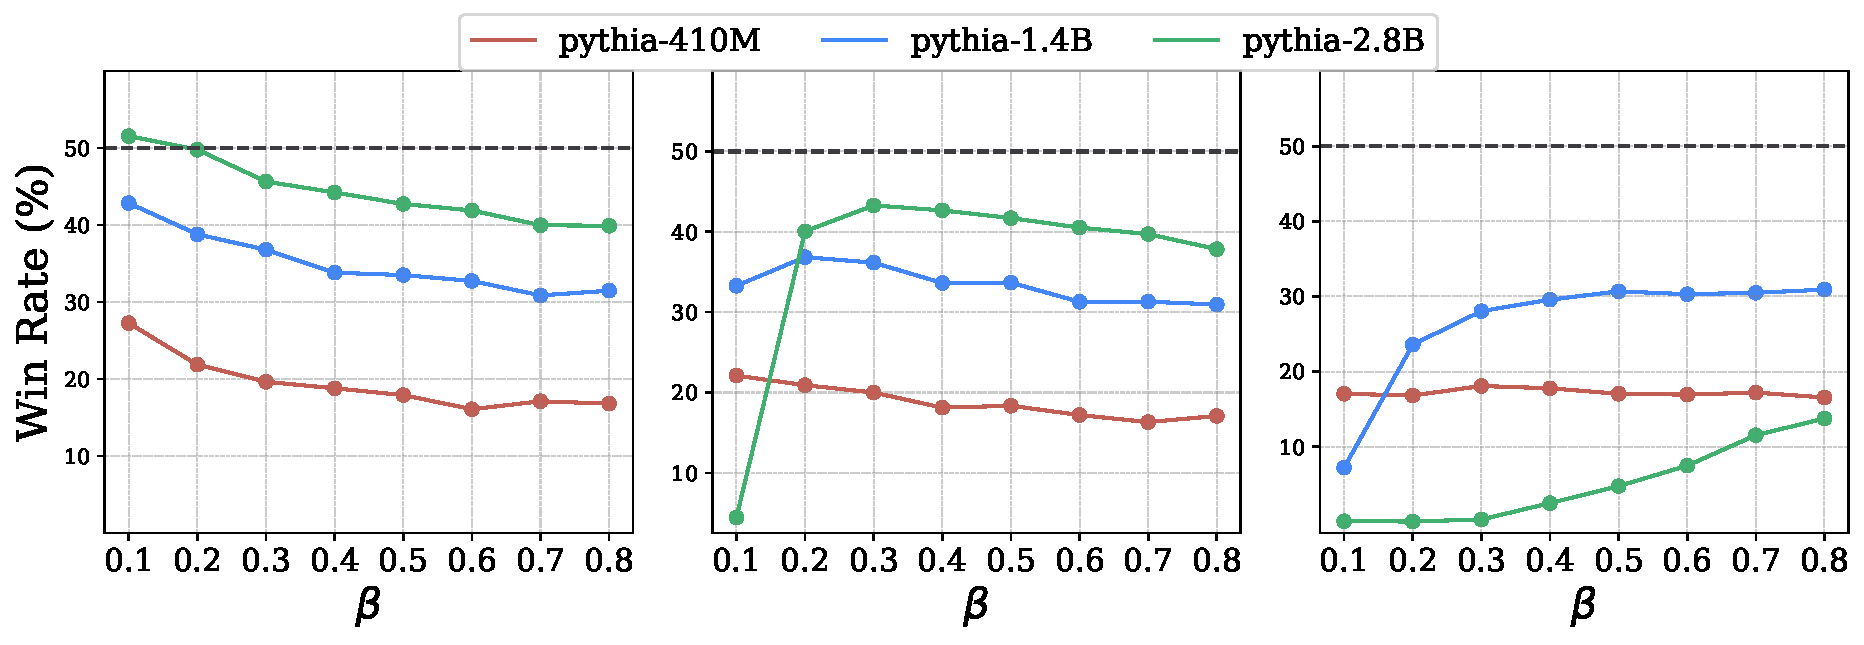
\includegraphics[width=1.0\linewidth]{figs/low_gap_mix_high_gap.pdf}
    % \vspace{-10pt}
    \caption{Win rate performance of DPO across different $\beta$ settings on the \emph{low gap}, \emph{mixed gap}, and \emph{high gap} datasets.}
    \label{fig_low_high_gap}
    \vspace{-10pt}
 \end{figure}
 
\textbf{Models and Metrics.} 
Our study evaluates various model sizes, specifically Pythia-410M, Pythia-1.4B, and Pythia-2.8B \cite{pythia}, to ensure a comprehensive assessment. Following the established protocol in DPO \cite{DPO}, each model iteration undergoes a single epoch with a batch size of 64. This setup provides a uniform basis for evaluation across different models.
We adopt the evaluation strategy from DPO \cite{DPO} to calculate the \textit{win rate}, a metric that measures how often the GPT-4 model prefers a response generated by our models over the default chosen response on the subset of the test dataset.

\textbf{Findings}: 
\textbf{(1) The optimal value of $\beta$ varies with data quality, reflecting divergent performance patterns across datasets.}
In Figure \ref{fig_low_high_gap}, we present the win rate results across three levels of pairwise data gap, each evaluated under varying $\beta$ parameters. As can be observed,
with \emph{low gap} pairwise data, a smaller $\beta$ value is preferable for optimizing performance. This is likely because the informative content of such data allows a lower $\beta$ to facilitate more substantial updates, thereby enhancing alignment accuracy.
Conversely, for \emph{high gap} pairwise data, maintaining a low $\beta$ may lead to overfitting, which significantly undermines the alignment process.
The \emph{mixed gap} dataset --- a combination of both \emph{low gap} and \emph{high gap} datasets --- exhibits a more nuanced performance pattern, suggesting the necessity for a dynamic $\beta$ calibration strategy to adapt to varying data quality.
Consequently, adhering to a fixed $\beta$ value, \ie configuring $\beta$ at the population level, might be inadequate for the dynamic and varied nature of real-world datasets.
\begin{wrapfigure}{r}{0.3\textwidth}
    \centering
    \vspace{-0.45cm}
    \!\!\!\!\!\!\!\! 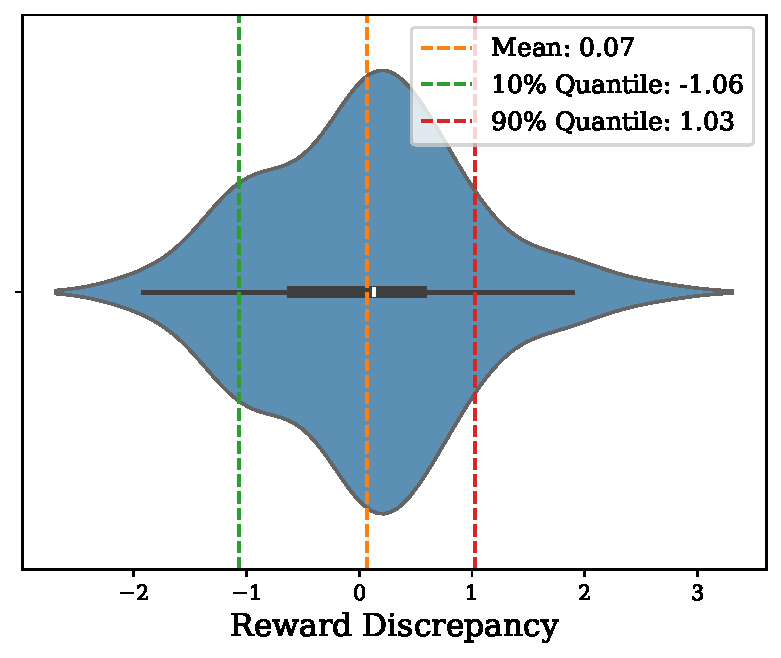
\includegraphics[width=0.32\textwidth]{figs/gap_distribution.pdf}
    \vspace{-0.3cm}
    \caption{The distribution of individual reward discrepancy ($r(\yb_w^{(i)};\xb^{(i)})-r(\yb_l^{(i)};\xb^{(i)})$) on the training dataset of HH.}
    \vspace{-0.5cm}
    \label{fig:gap_distribution}
  \end{wrapfigure}
\textbf{(2) The dataset exhibits notable outliers.} In Figure \ref{fig:gap_distribution}, utilizing the Pythia-2.8B model, we evaluate the data quality by examining the distribution of reward discrepancy for each triplet (which we will define as ``individual reward discrepancy'' later) within the HH dataset's training samples. 
The tails of the density plot extend beyond the highlighted percentiles, suggesting the existence of data samples with significantly higher or lower reward discrepancies.
Notably, cases with significantly higher rewards for positive samples over negative ones suggest low informational value, as these discrepancies likely do not contribute meaningfully to the model's learning process. Whereas the opposite cases hint at potential labeling errors. Both cases deviate from an expected rational distribution range and are thus classified as outliers. For further details on outliers, kindly refer to Appendix \ref{low_gap_high_gap}.

\subsection{Method: Dynamic $\beta$ Calibration in DPO}

Through our empirical analysis, we highlight the sensitivity of DPO to $\beta$ selections and the frequent occurrence of outliers. Hence, 
determining the optimal $\beta$ value requires careful consideration of the quality of pairwise data while also addressing the influence of outliers. This prompts the question: \textit{what criteria define a superior choice of $\beta$?} In response, we propose the following guiding principles:

\textbf{Principle 1:} \textit{The optimal $\beta$ value should be responsive to pairwise data's quality.}

\textbf{Principle 2:} \textit{The selection of $\beta$ value should minimize the influence of outliers.}

\subsubsection{Dynamic $\beta$ Calibration at Batch-Level}
We begin by introducing the concept termed `\textit{individual reward discrepancy}', which represents the difference between the rewards of winning and losing for each triplet, serving as a measurement for pairwise data quality. Formally, for a triplet $(\xb^{(i)}, \yb_w^{(i)}, \yb_l^{(i)}) \in \Set{D}$, the individual reward discrepancy is defined as 
$M_i = r(\yb_w^{(i)};\xb^{(i)}) - r(\yb_l^{(i)};\xb^{(i)}).$
While our primary analysis utilizes the implicit reward model induced by the policy trained using DPO, we also conducted comparative experiments with an explicit reward model. The details of these experiments with the explicit RM can be found in Appendix \ref{sec:appendix_explicit_rm}. For the DPO-based implicit reward model, the reward discrepancy is expressed as:
% To clarify how the reward model is constructed and used, we directly use the implicit reward model induced by the policy trained using DPO. Specifically, the reward discrepancy in DPO is expressed as:

$$ M = \beta_0 \log \left( \frac{\pi_\theta (y_w \mid x) }{\pi_{\text{ref}}(y_w \mid x)} \right) - \beta_0 \log \left( \frac{\pi_\theta (y_l \mid x) }{\pi_{\text{ref}}(y_l \mid x)} \right). $$

Here, \(\pi_\theta\) represents the policy being optimized, and \(\pi_{\text{ref}}\) denotes the reference policy. This formulation captures the difference in the log-probabilities of the winning and losing outcomes, weighted by the parameter \(\beta\).
Motivated by our guiding principles, a straightforward approach is to assign a distinct $\beta$ to each triplet, allowing each $\beta$ to serve as a parameter tailored to its respective triplet. This instance-level dynamic $\beta$ adaption can be formulated as follows:

\begin{eqnarray}
    \begin{aligned}
        \beta_i = \beta_0 + \alpha \large(M_i - M_0 \large) \beta_0 = [1 + \alpha(M_i-M_0)]\beta_0,
    \end{aligned}
    \label{eq:beta}
\end{eqnarray}

where $\beta_0$ represents the benchmark hyperparameter intrinsic to DPO, typically set to 0.1. The term $M_0$ denotes a predetermined threshold, and the coefficient $\alpha$ is a scaling factor within the interval $[0, 1]$ that adjusts the influence of $M_i$ on $\beta_i$. Specifically, when $\alpha = 0$, $\beta_i$ remains constant at $\beta_0$, thus maintaining the standard DPO framework without modification.
% We begin by introducing the concept termed `\textit{individual reward discrepancy}', which represents the difference between the rewards of winning and losing for each triplet, serving as a measurement for pairwise data quality.
% Formally, for a triplet $(\xb^{(i)}, \yb_w^{(i)}, \yb_l^{(i)}) \in \Set{D}$, the individual reward discrepancy is defined as $M_i = r(\yb_w^{(i)};\xb^{(i)})-r(\yb_l^{(i)};\xb^{(i)})$.
% Motivated by our guiding principles, a straightforward approach is to assign a distinct $\beta$ to each triplet, allowing each $\beta$ to serve as a parameter tailored to its respective triplet. This instance-level dynamic $\beta$ adaption can be formulated as follows:
% \begin{eqnarray}
%     \begin{aligned}
%         \beta_i = \beta_0 + \alpha \large(M_i - M_0 \large) \beta_0 = [1 + \alpha(M_i-M_0)]\beta_0,
%     \end{aligned}
%     \label{eq:beta}
% \end{eqnarray}
% where $\beta_0$ represents the benchmark hyperparameter intrinsic to DPO, typically set to 0.1. The term $M_0$ denotes a predetermined threshold, and the coefficient $\alpha$ is a scaling factor within the interval $[0, 1]$ that adjusts the influence of $M_i$ on $\beta_i$. Specifically, when $\alpha = 0$, $\beta_i$ remains constant at $\beta_0$, thus maintaining the standard DPO framework without modification.

Equation \eqref{eq:beta} illustrates that $\beta_i$ increases monotonically with $M_i$, allowing the model to adjust the $\beta$ value based on the running reward differential between paired samples.\
Nevertheless, such instance-level adjustments may introduce instabilities during training. Prior studies have shown that a minibatch approach can help avoid saddle points or local minima \cite{ge2015escaping}, as well as mitigate the impact of noise \cite{robbins1951stochastic, bottou2010large}. Drawing inspiration from these benefits, we propose a batch-level dynamic estimation methodology for $\beta$:

\begin{equation}
    \beta_{\text{batch}} = [1 + \alpha( \EE_{i \sim \text{batch}}[M_i]-M_0)]\beta_0.
\end{equation}
In practical applications, the threshold $M_0$ can be estimated by employing the global mean of $M_i$ with a moving average updating scheme \cite{mae}:
\begin{equation}
    M_0  \leftarrow m M_0 + (1-m)  \EE_{i \sim \text{batch}}[M_i],
    \label{mom}
\end{equation}
where $m\in[0,1)$ is a momentum coefficient.
Such a batch-level calibration method introduces only one new parameter, $\alpha$, to control the scale of $\beta$ adjustment.
The calculation of $\EE_{i \sim \text{batch}}[M_i]$ is straightforward within DPO procedures, thereby incurring no additional computational overhead.


\subsubsection{$\beta$-Guided Data Filtering }
To mitigate the adverse impact of outliers on the $\beta$ selection process, we introduce a $\beta$-guided data filtering mechanism. Informed by $3\sigma$ confidence criterion \cite{3sigma}, this strategy employs a probabilistic model to assess the significance of each triplet $(\xb^{(i)}, \yb_w^{(i)}, \yb_l^{(i)})$ based on its individual reward discrepancy $M_i$, which is defined as:
\begin{equation}
    p(M_i) = \frac{1}{\sqrt{2\pi}\sigma} \exp\left(-\frac{(M_i-M_0)^2}{2\sigma^2}\right),
    \label{sampling_p}
\end{equation}
where $M_0$ and $\sigma$ represent the mean and standard deviation of $M_i$ across the training dataset, respectively.
Similar to the updating scheme of $M_0$ in Equation \eqref{mom}, we dynamically estimate the value of $\sigma$ using the moving average method:
\begin{equation}
     \sigma \leftarrow m \sigma + (1-m)  \sqrt{\mathbb{V}_{i \sim\text{batch}}[M_i]}.
     \label{mom2}
\end{equation}
This probabilistic weighting discerns the relative importance of each sample, guiding the selection of $|\text{batch}| \times \rho$ samples (without replacement) based on their calculated probabilities $p(M_i)$. Here, $\rho$ denotes the selection ratio, defaulting to 0.8, a choice validated by preliminary experiments aimed at optimizing training efficiency and model accuracy.

This process is iterated for each training batch, ensuring that the training data is continuously updated to reflect the most informative samples. The introduction of the $\beta$-guided data filtering strategy is instrumental in fortifying the model against outliers, thereby facilitating the accurate estimation of the $\beta$ value.

\textbf{Highlights:}
We underline the following key features of our proposed $\beta$-DPO framework:
\begin{itemize}[leftmargin=*]
    \item \textbf{Simplicity}: $\beta$-DPO is extremely straightforward and quick to implement. It merely involves a dynamic $\beta$ adjustment at the batch level and a $\beta$-guided data filtering mechanism, both of which are predicated upon the reward discrepancy denoted by $M_i$.
    \item \textbf{Efficiency}: Unlike other methodologies \cite{RSO,morimura2024filtered,pruthi2020estimating,f-dpo} that necessitate an additional gold model for data filtering, our method leverages the running reward discrepancy $M_i$ within the DPO framework. Moreover, our empirical studies indicate that $\beta$-DPO exhibits insensitivity to the hyperparameters $\rho$. A default setting of $\rho=0.8$ typically yields satisfactory performance.
    \item \textbf{Model-agnostic}: As a variant of the traditional DPO, the proposed $\beta$-DPO can function as a plug-and-play module. It allows straightforward integration of future enhancements and extensions within the DPO framework. Our empirical investigations corroborate this assertion.
\end{itemize}

\subsection{Discussion with Previous Studies}
\textbf{Relations to Data Selection.} An increasing volume of works \cite{RSO,morimura2024filtered,LIMA,pruthi2020estimating, xia2024less} have underscored the impact of data quality on the performance of LLM's alignment. A common practice among these efforts involves employing a so-called ``gold model'' for data selection. This approach, however, introduces significant computational demands and the choice of the gold model directly influences the resultant system's performance. The focus of this work, it should be noted, is not to propose a superior strategy for data selection. Instead, we aim to enhance adaptability to the quality of data by dynamically adjusting the $\beta$ parameter. This adjustment facilitates improved $\beta$ estimation by selecting data based on the reward. Moreover, Section \ref{exp_adaptation} illustrates the compatibility of dynamic $\beta$ adjustment with other data selection methodologies.

\textbf{Relations to Recent Temperature Schemes.}
Dynamic temperature frameworks have been introduced in the realm of contrastive learning, motivated by various objectives, such as addressing out-of-distribution tasks \cite{Uncertainty} or accommodating long-tail data distributions \cite{long_tail}. The work most closely related to ours, MACL \cite{MACL}, has indeed proposed an alignment-adaptive strategy; however, its primary aim was to navigate the uniformity-tolerance dilemma. Hence, the integration of dynamic temperature mechanisms with LLM's alignment remains an underexplored area against this backdrop.